
	
	W tym rozdziale zostanie opisany plan pracy nad robotem, który powinien doprowadzić do zbudowania robota oraz aplikacji przedstawionych w opisie projektu.
	
	\subsection{Kamienie milowe}
	
	Poniżej zostały przedstawione główne kroki, które należy wykonać aby zakończyć pracę nad projektem z oczekiwanymi rezultatami.
	
	\begin{table}[h]
	\centering
		\begin{tabularx}{0.8\linewidth}{|c|X|}
			\hline
			Lp. & Opis \\ \hline
			1  & Zbudowanie podwozia robota \\ \hline
			2  & Umieszczenie potrzebnej elektroniki - mikrokontroler, czujniki, serwomechanizm  \\ \hline
			3 & Oprogramowanie robota \\ \hline
			4 & Zakończenie pracy nad aplikacją na komputery osobiste do generowanie mapy otoczenia \\ \hline
			5 & Połączenie pracy robota i aplikacji \\ \hline
		\end{tabularx}
		\caption{Table opisująca poszczególne kamienie milowe}
	\end{table}
\subsection{Szczegółowy plan pracy}
	
	Poniżej został przedstawiony szczegółowy plan pracy nad projektem.
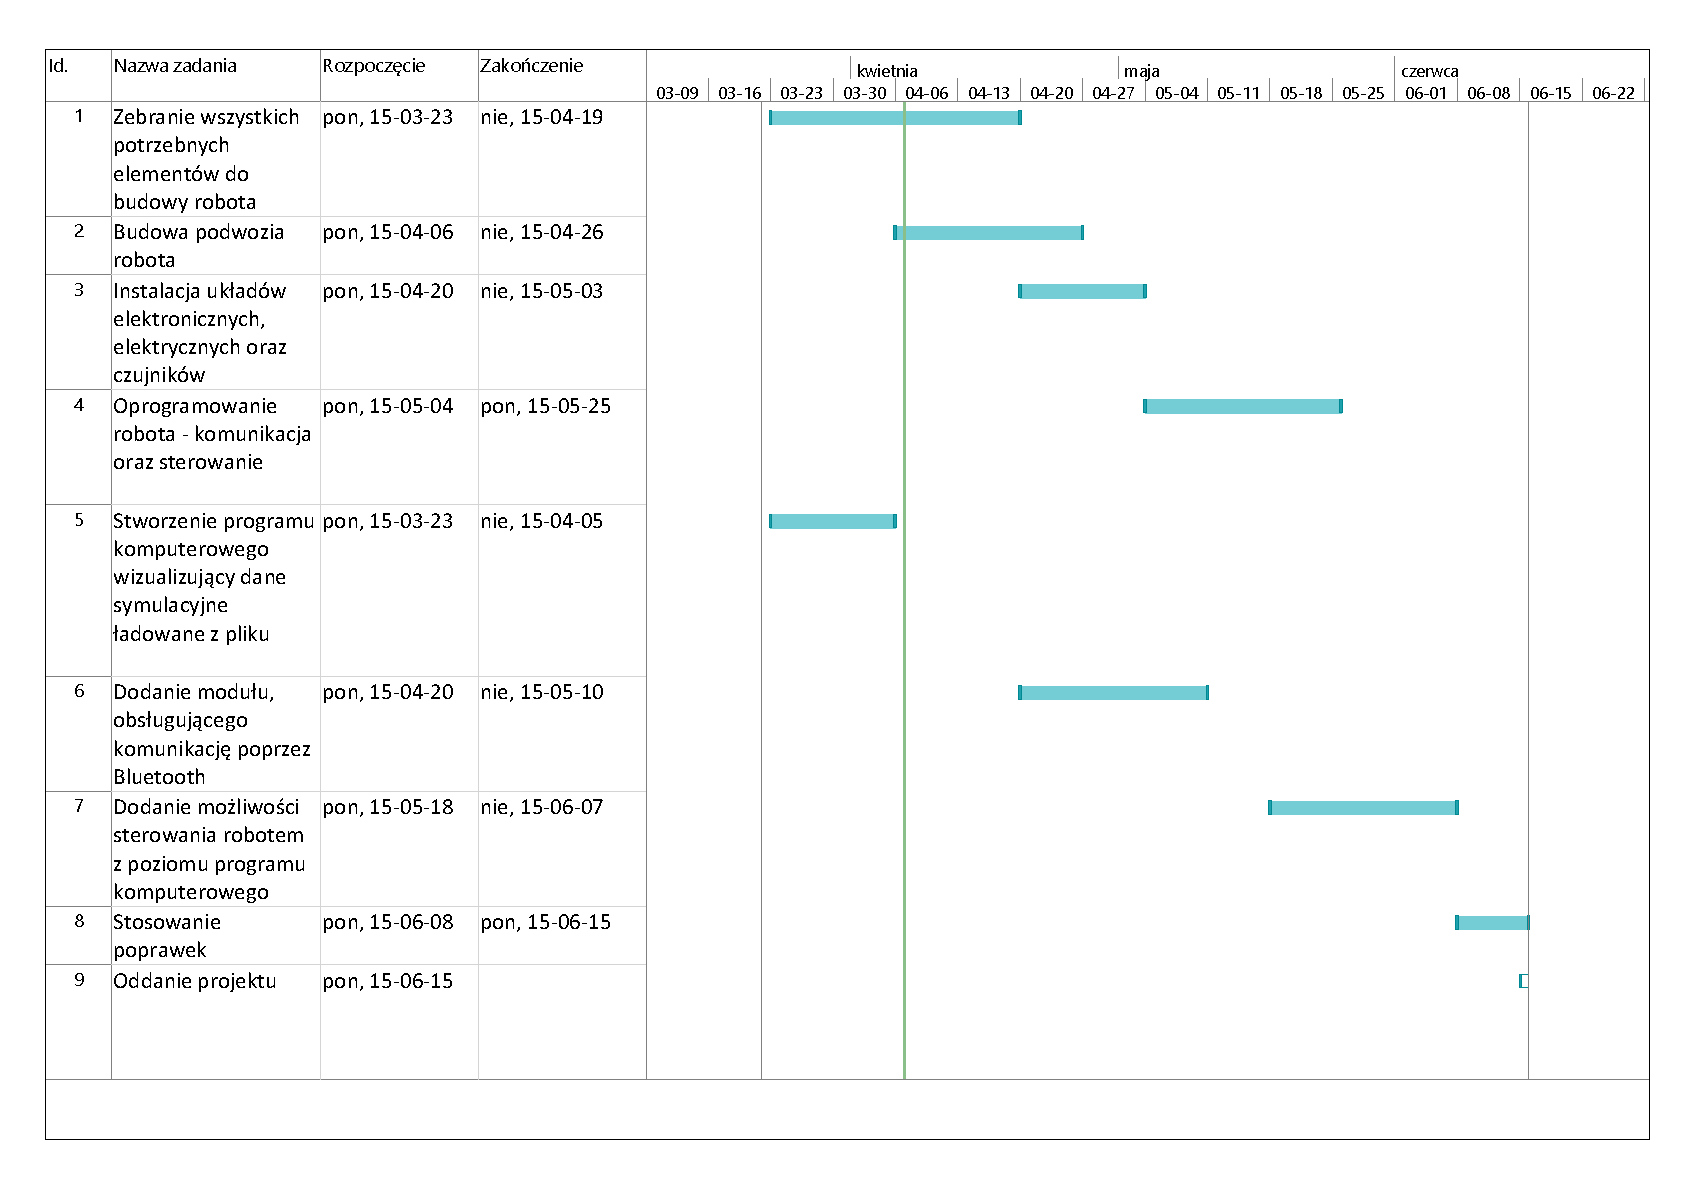
\includepdf[pages={1}, landscape]{MS_Project.pdf}
	
	

